%!TEX root = ../Thesis.tex
\section*{Anhang}
\addcontentsline{toc}{section}{Anhang}
\fancyhead[R]{Anhang}

\anhangsverzeichnis

\anhang{Testdurchführung \textcolor{blue}{[Julius Figge]}}

\begin{center}
    \label{fig:testdurchf}
    \begin{longtable}{|p{0.4\textwidth}|p{0.3\textwidth}|p{0.2\textwidth}|}
        \caption{GUI-Testdurchführung}\\
        \hline
        Aktion & erwartetes Ergebnis & Reaktion\\
        \hline
        \hline

        \textbf{Registrieren eines neuen Nutzers} & &\\
        \hline
        Bereits bestehenden Nutzernamen verwenden (admin) & Fehlermeldung - Nutzername existiert bereits &\\
        \hline
        zu kurzer Nutzername (<3) & Fehlermeldung - Daten falsch &\\
        \hline
        zu kurzes Passwort (<=7) & Fehlermeldung - zu kurzes Passwort &\\
        \hline
        nicht übereinstimmende Passwörter & Fehlermeldung - nicht stimmende Passwort &\\
        \hline
        mit korrekten Daten & eingeloggt sein &\\
        \hline
        \hline

        \textbf{Ausloggen aus dem Account} & ausgeloggt sein &\\
        \hline
        \hline

        \textbf{Einloggen in erstellten Account} & &\\
        \hline
        mit falschem Passwort & Fehlermeldung &\\
        \hline
        mit falschem Nutzernamen & Fehlermeldung &\\
        \hline
        mit richtigem Passwort & eingeloggt sein &\\
        \hline
        \hline

        \textbf{Erstellen von beispielhaften Ideen} & &\\
        \hline
        Erstellen einer \enquote{internen Idee} & Idee erscheint in Tabelle nicht eingereichter Ideen &\\
        \hline
        Erstellen einer \enquote{Produkt-Idee} & Idee erscheint in Tabelle nicht eingereichter Ideen &\\
        \hline
        Erstellen einer beliebigen Idee mit fehlerhaften Werten & Fehlerhafte Attribute werden hervorgehoben &\\
        \hline
        Erstellen einer Idee von der bereits selber Name bei selbem Typ vorhanden & Fehlermeldung über Duplikat &\\
        \hline
        Bearbeitend der internen Idee & Änderungen werden übernommen &\\
        \hline
        Bearbeitend der Produkt-Idee & Änderungen werden übernommen &\\
        \hline
        \hline

        \textbf{Ideenübersicht} & &\\
        \hline
        Filtern der nicht eingereichten Ideen nach Attributen & nur Ideen mit passenden Attributen werden angezeigt &\\
        \hline
        Einreichen der erstellten Ideen & erfolgreicher Transfer in jeweilige Tabelle &\\
        \hline
        \hline

        \textbf{Ausloggen aus dem Account} & ausgeloggt sein &\\
        \hline
        \hline

        \textbf{Idee Übersicht als nicht eingeloggter Nutzer} & &\\
        \hline
        Filtern der Ideen in beiden Tabellen & nur Ideen mit passenden Attributen werden angezeigt &\\
        \hline
        \hline

        \textbf{Spezialist für \enquote{internen Idee}} & &\\
        \hline
        Einloggen als passender (Ideen sollten ihm zugewiesen sein) Spezialist (Zugangsdaten siehe \texttt{Manual.md})& eingeloggt sein &\\
        \hline
        Übersicht zu entscheidender Ideen filtern & nur Ideen mit passenden Attributen werden angezeigt &\\
        \hline
        Entscheiden ohne Begründung & fehlendes Attribut wird hervorgehoben &\\
        \hline
        Idee in Ideenspeicher verschieben & Idee liegt in Ideenspeicher &\\
        \hline
        \hline

        \textbf{Spezialist für \enquote{Produkt-Idee}} & &\\
        \hline
        Account zu anderem Spezialist wechseln & Idee liegt in Ideenspeicher &\\
        \hline
        Entscheiden über Idee aus Ideenspeicher mit Auswahl  \enquote{zur Entscheidung freigegeben} & Idee liegt in eigenen zu entscheidenden Ideen &\\
        \hline
        Idee aus Entscheidungsübersicht bewerten & Idee erscheint auf passender Tabelle in Ideenübersicht &\\
        \hline
        \hline

        \textbf{Administrator} & &\\
        \hline
        Account zu Administrator wechseln (Zugangsdaten siehe \texttt{Manual.md})& &\\
        \hline
        Existierende User prüfen & registrierter Account sowie alle Spezialisten werden aufgelistet &\\
        \hline
        Alle möglichen anzulegenden Felder durchgehen, bereits bestehenden Namen eingeben & bei jedem Feld wird ein Fehler angezeigt &\\
        \hline
        Alle möglichen anzulegenden Felder durchgehen & Feld wird angelegt &\\
        \hline
        Ausloggen & \textbf{FERTIG!} &\\
        \hline
    \end{longtable}
\end{center}

\clearpage
\pagebreak

\anhang{Weitere Use-Cases \textcolor{blue}{[Julius Figge]}}\label{Anhang-Use-Cases}

\subanhang{Administrator}\label{Anhang-Admin}
\begin{figure}[h]
    \centering
    \begin{minipage}[t]{1\textwidth}
        \caption{Administrator - Use-Case Diagramm}
        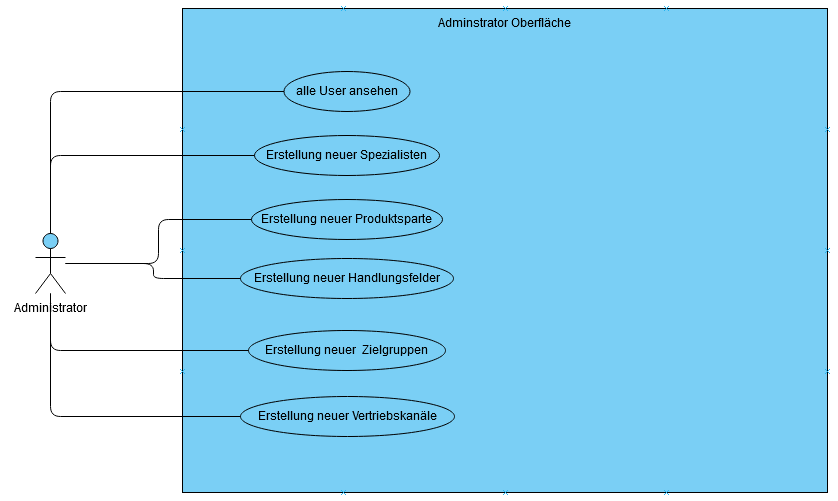
\includegraphics[width=1\textwidth]{img/admin-use-case.png}\\
        \source{Eigene Darstellung}
    \end{minipage}
\end{figure}

\subanhang{Kontaktformular}\label{Anhang-Kontakt}
\begin{figure}[h]
    \centering
    \begin{minipage}[t]{1\textwidth}
        \caption{Kontaktformular - Use-Case Diagramm}
        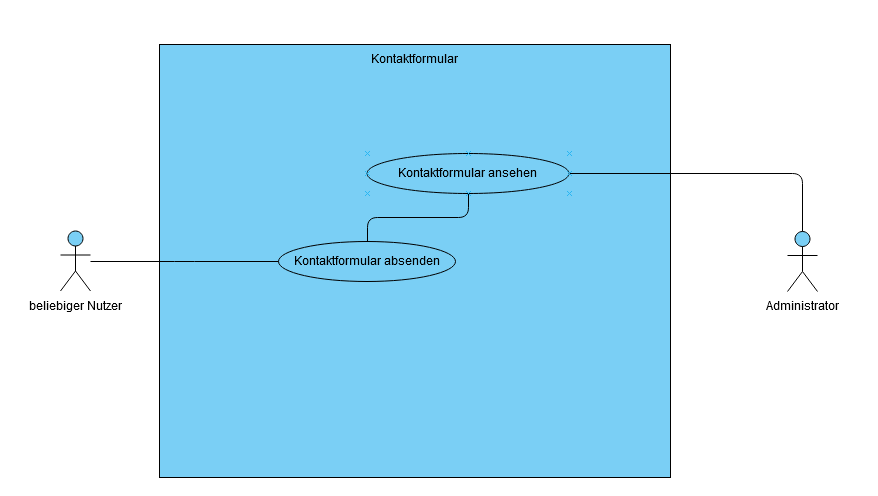
\includegraphics[width=1\textwidth]{img/kontakt-use-case.png}\\
        \source{Eigene Darstellung}
    \end{minipage}
\end{figure}

\clearpage
\pagebreak

\anhang{GUI-Konzept \textcolor{blue}{[Julius Figge]}}

\subanhang{Konzept}\label{GUI-Konzept}

\begin{figure}[hbt]
    \centering
    \begin{minipage}[t]{1\textwidth}
        \caption{GUI-Konzept - Login}
        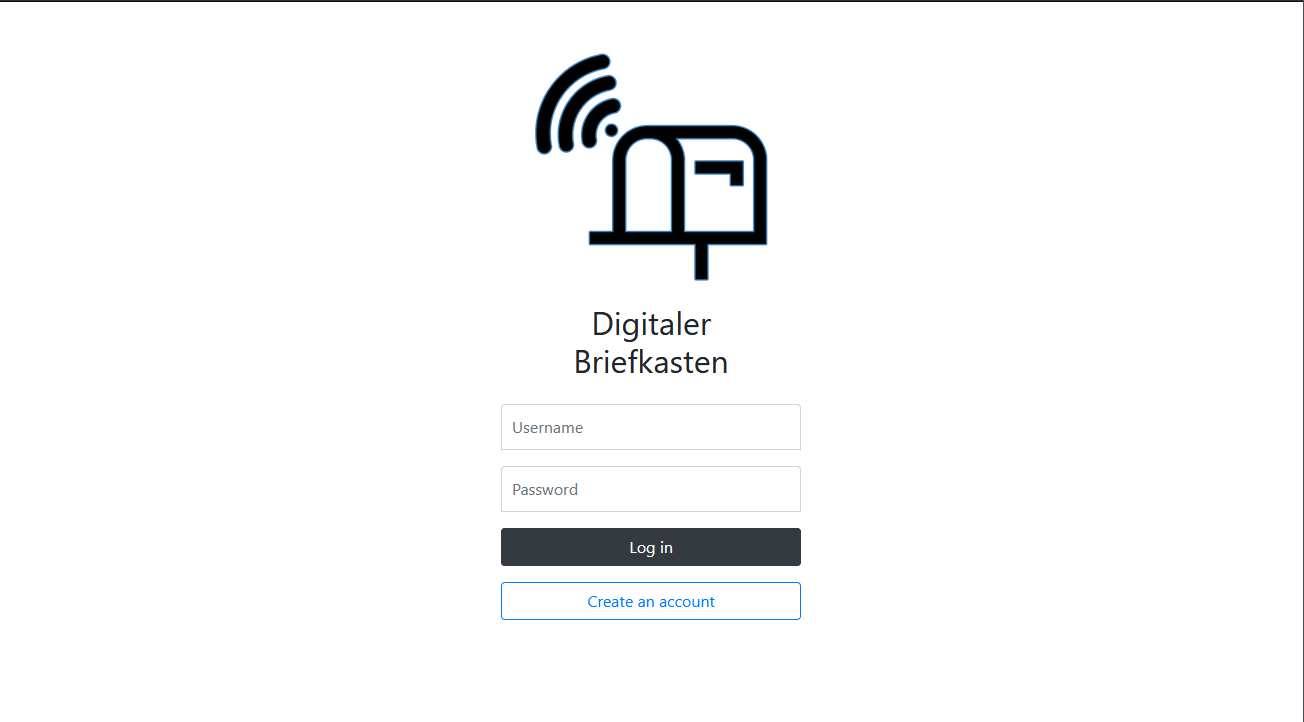
\includegraphics[width=1\textwidth]{img/login-konzept.png}\\
        \source{Eigene Darstellung}
        \label{fig:login}
    \end{minipage}
\end{figure}

\begin{figure}[h]
    \centering
    \begin{minipage}[t]{1\textwidth}
        \caption{GUI-Konzept - Registrierung }
        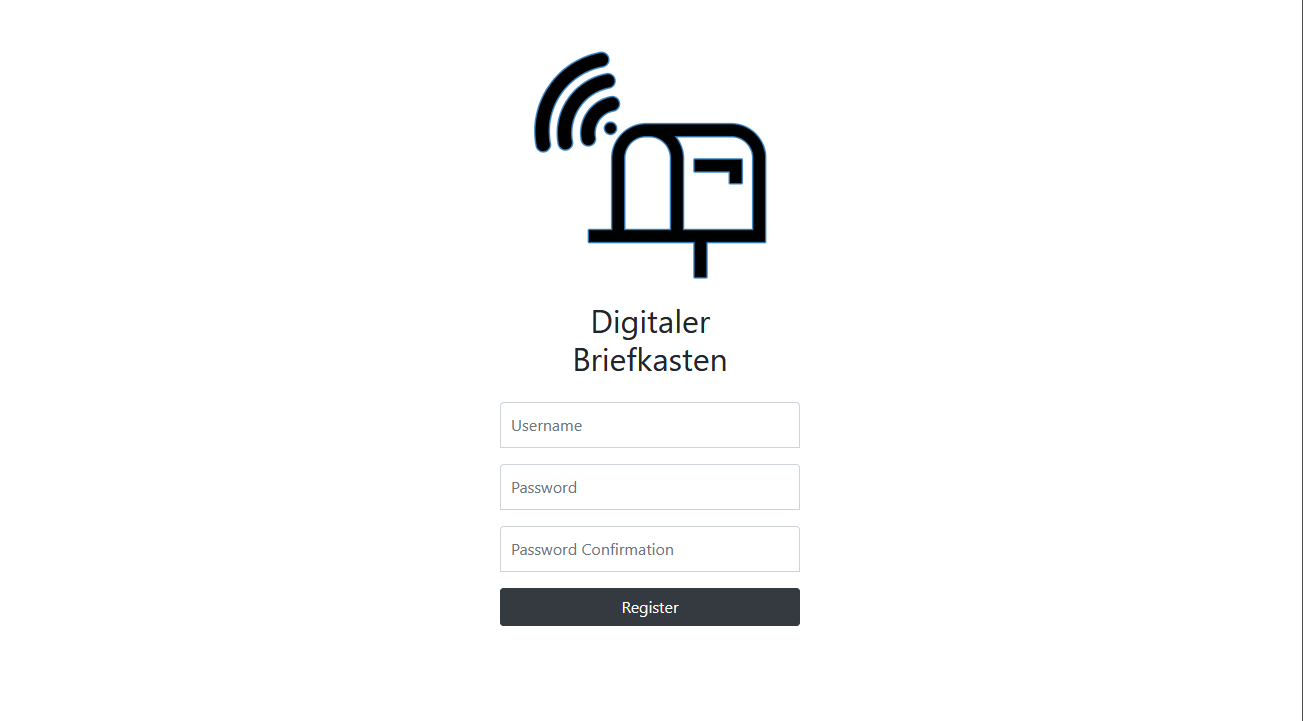
\includegraphics[width=1\textwidth]{img/registrierung-konzept.png}\\
        \source{Eigene Darstellung}
    \end{minipage}
\end{figure}

\begin{figure}[h]
    \centering
    \begin{minipage}[t]{1\textwidth}
        \caption{GUI-Konzept - Willkommen}
        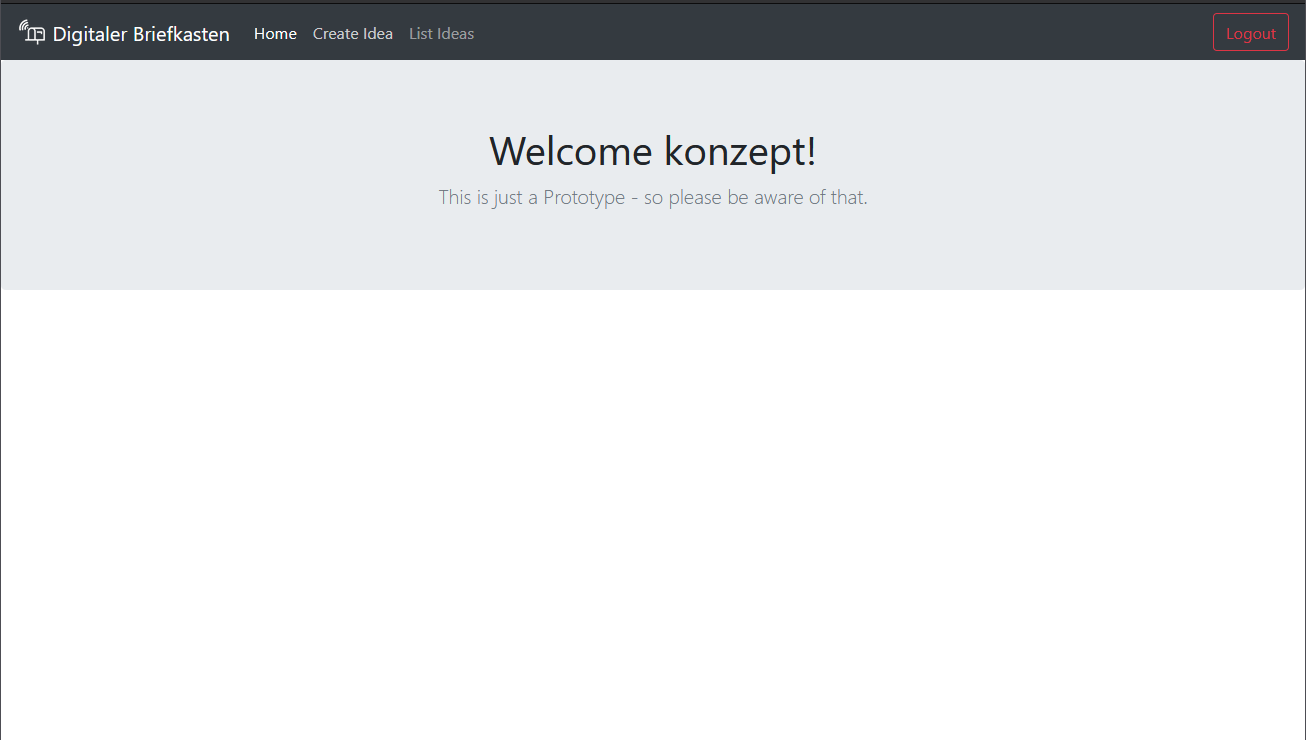
\includegraphics[width=1\textwidth]{img/welcome-konzept.png}\\
        \source{Eigene Darstellung}
    \end{minipage}
\end{figure}

\begin{figure}[h]
    \centering
    \begin{minipage}[t]{1\textwidth}
        \caption{GUI-Konzept - Idee erstellen }
        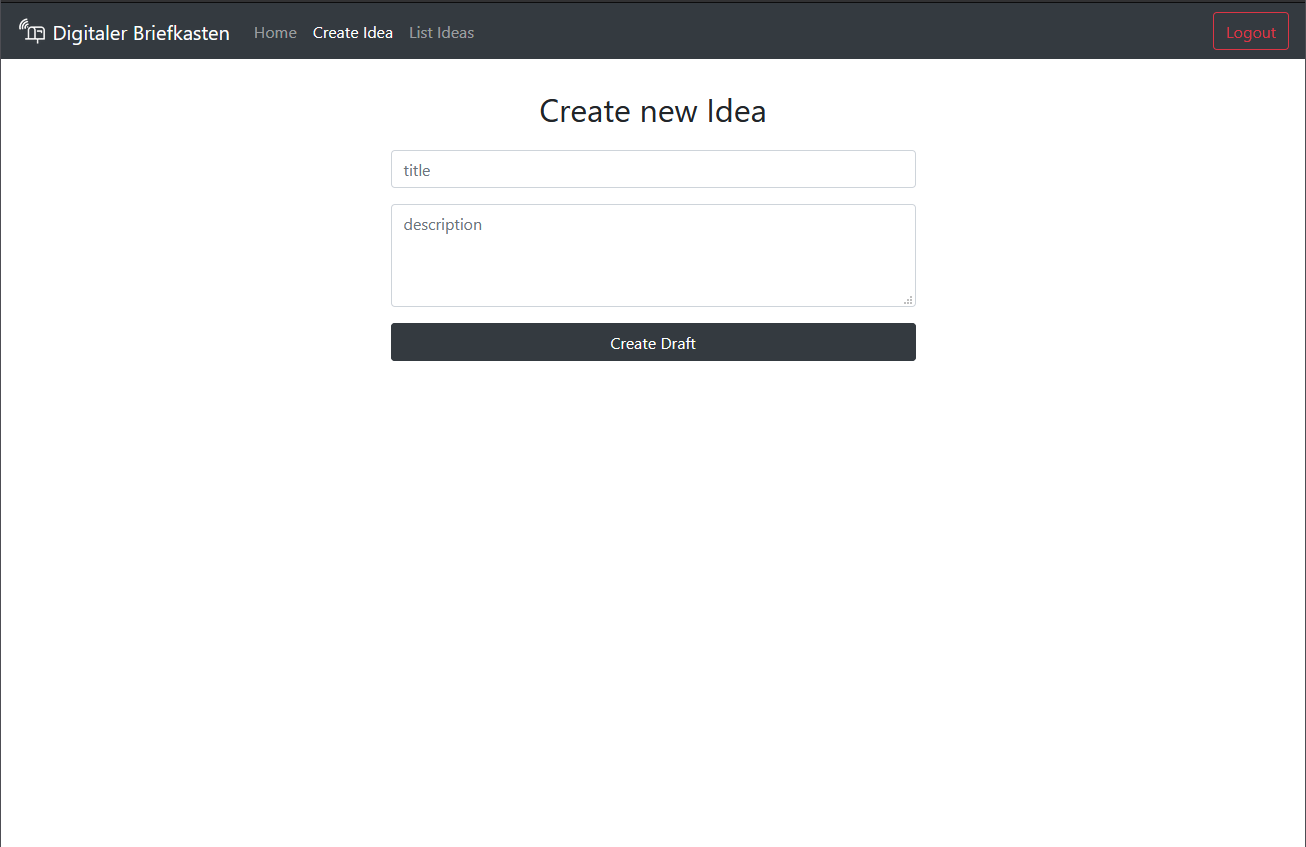
\includegraphics[width=1\textwidth]{img/createIdea-konzept.png}\\
        \source{Eigene Darstellung}
    \end{minipage}
\end{figure}

\clearpage
\pagebreak

\subanhang{Umsetzung}\label{GUI-Umsetzung}

Die im folgenden dargestellten GUI Bestandteile stellen die wichtigsten Teile der Oberfläche dar. Auf die Abbildung aller Bestandteile wurde aufgrund der zu großen Menge, zur Wahrung der Übersichtlichkeit, verzichtet.

\begin{figure}[h]
    \centering
    \begin{minipage}[t]{1\textwidth}
        \caption{GUI-Umsetzung - Login }
        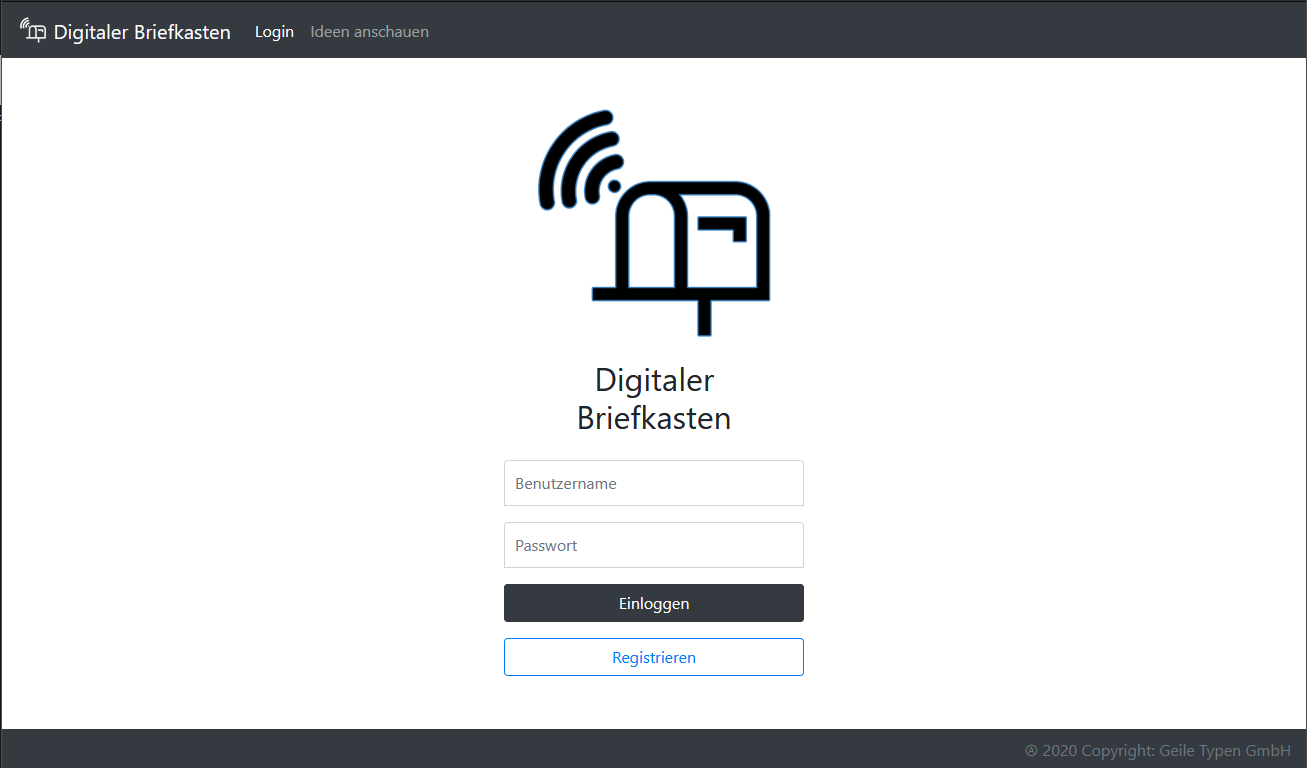
\includegraphics[width=1\textwidth]{img/login-umsetzung.png}\\
        \source{Eigene Darstellung}
    \end{minipage}
\end{figure}

\begin{figure}[h]
    \centering
    \begin{minipage}[t]{1\textwidth}
        \caption{GUI-Umsetzung - Registrierung }
        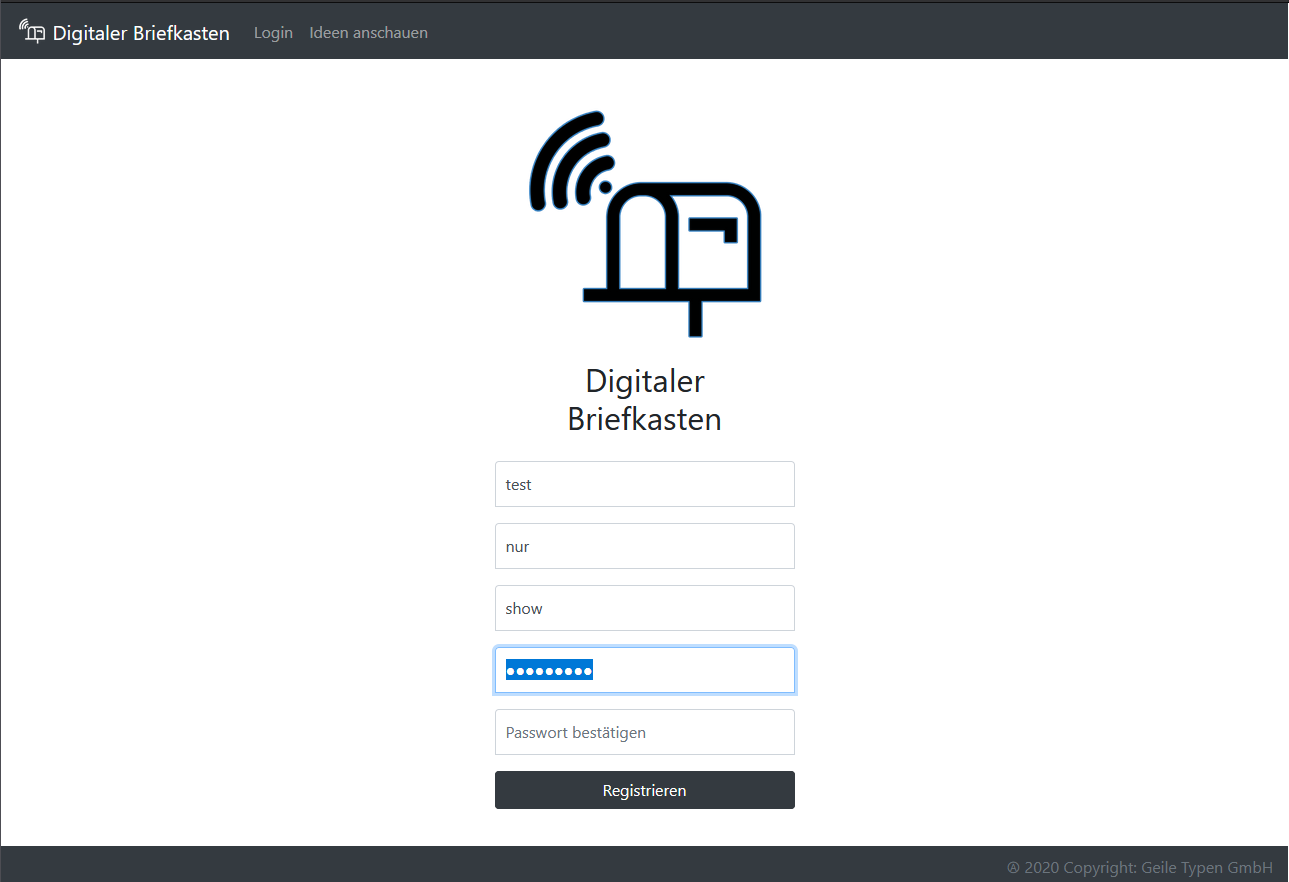
\includegraphics[width=1\textwidth]{img/registrierung-umsetzung.png}\\
        \source{Eigene Darstellung}
    \end{minipage}
\end{figure}

\begin{figure}[h]
    \centering
    \begin{minipage}[t]{1\textwidth}
        \caption{GUI-Umsetzung - Ideen}
        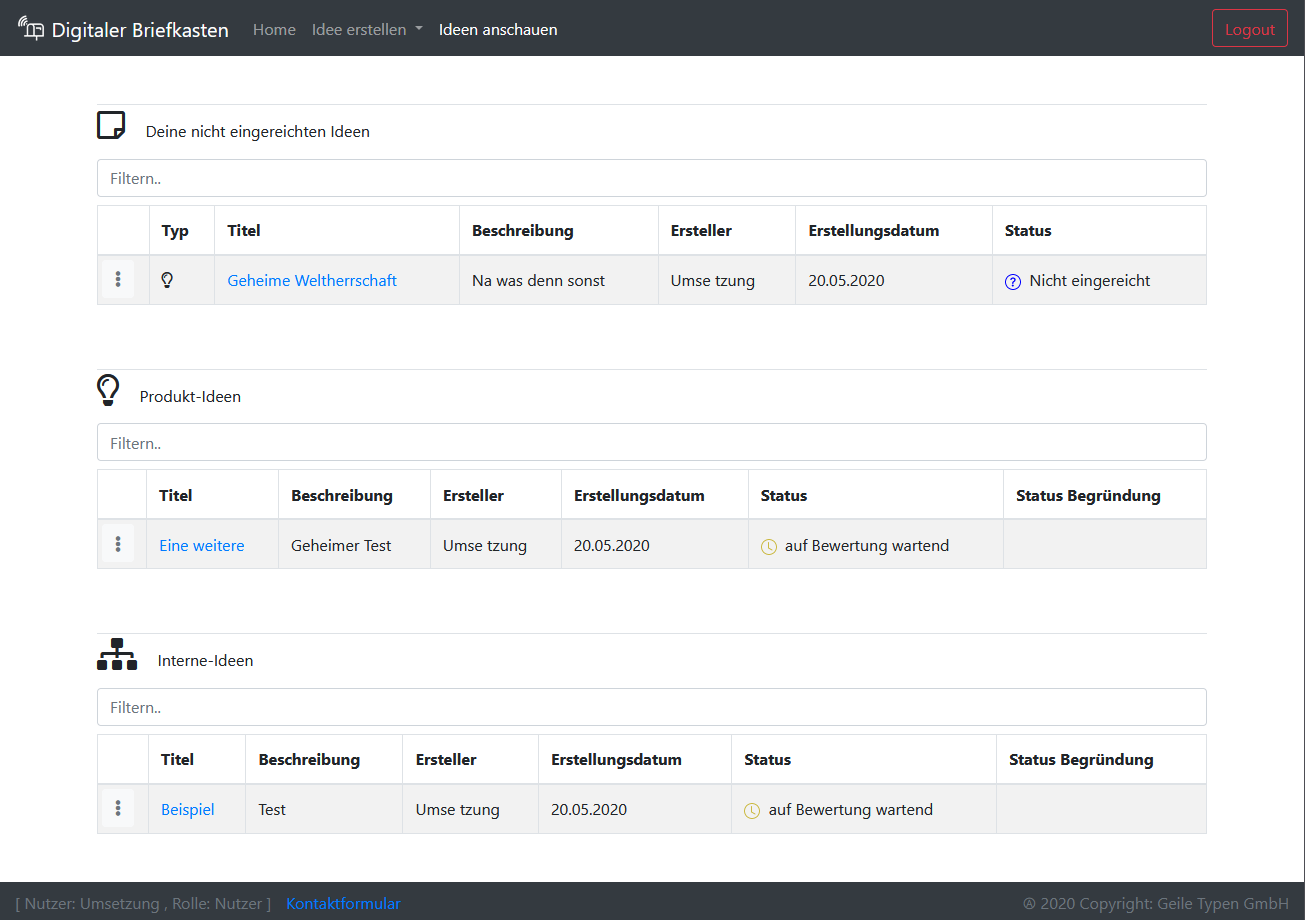
\includegraphics[width=1\textwidth]{img/ideen-umsetzung.png}\\
        \source{Eigene Darstellung}
    \end{minipage}
\end{figure}

\begin{figure}[h]
    \centering
    \begin{minipage}[t]{1\textwidth}
        \caption{GUI-Umsetzung - Idee erstellen }
        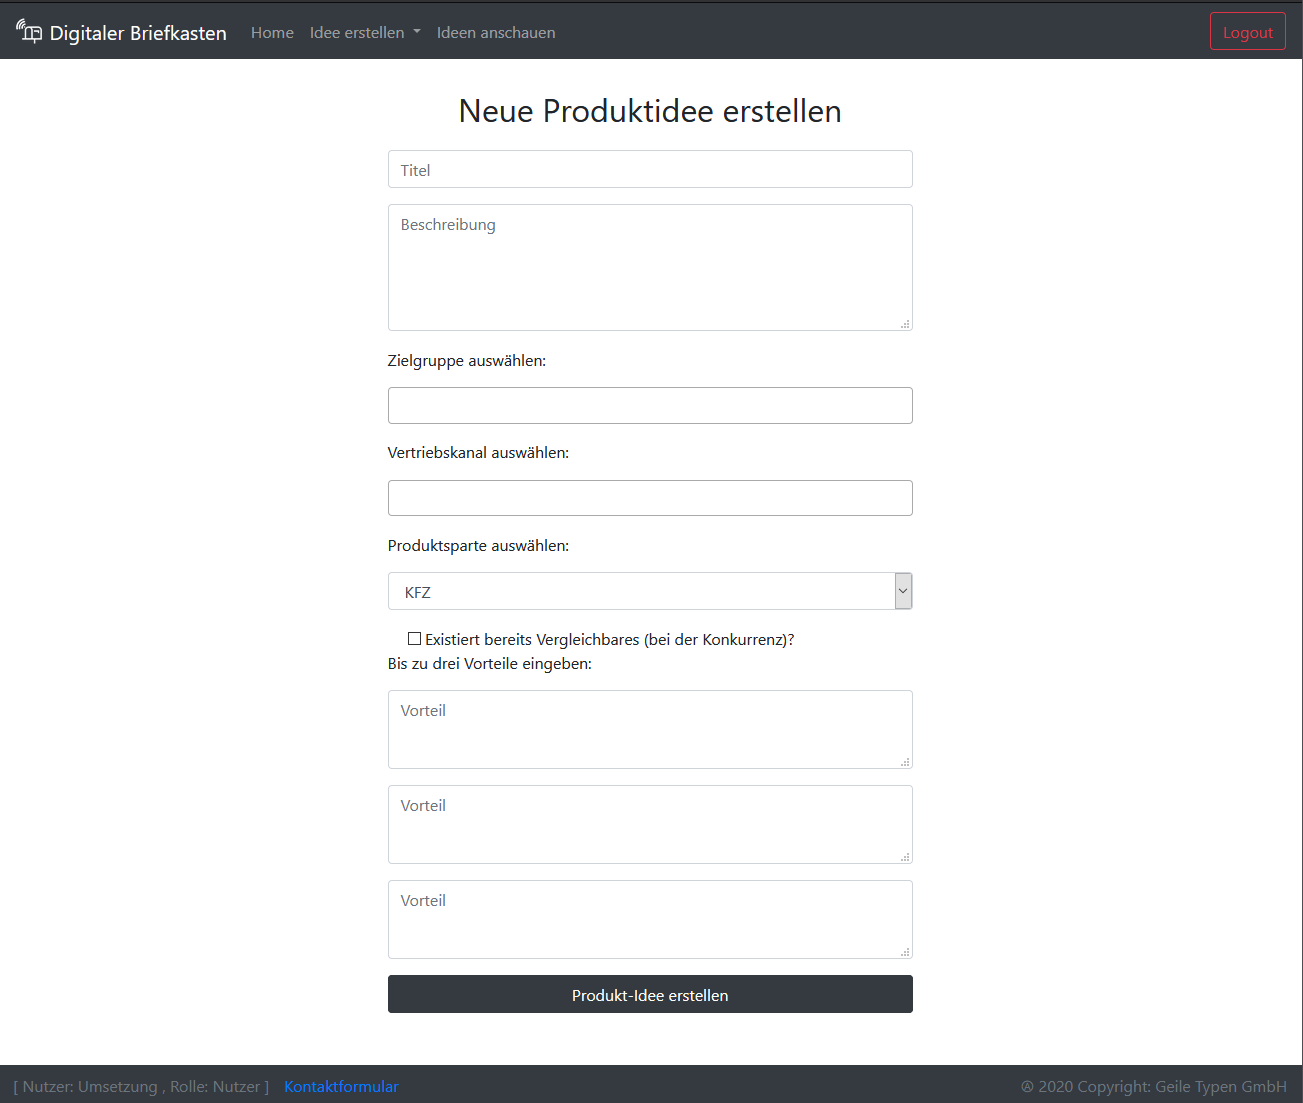
\includegraphics[width=1\textwidth]{img/createIdea-umsetzung.png}\\
        \source{Eigene Darstellung}
    \end{minipage}
\end{figure}

\begin{figure}[h]
    \centering
    \begin{minipage}[t]{1\textwidth}
        \caption{GUI-Umsetzung - Idee ansehen }
        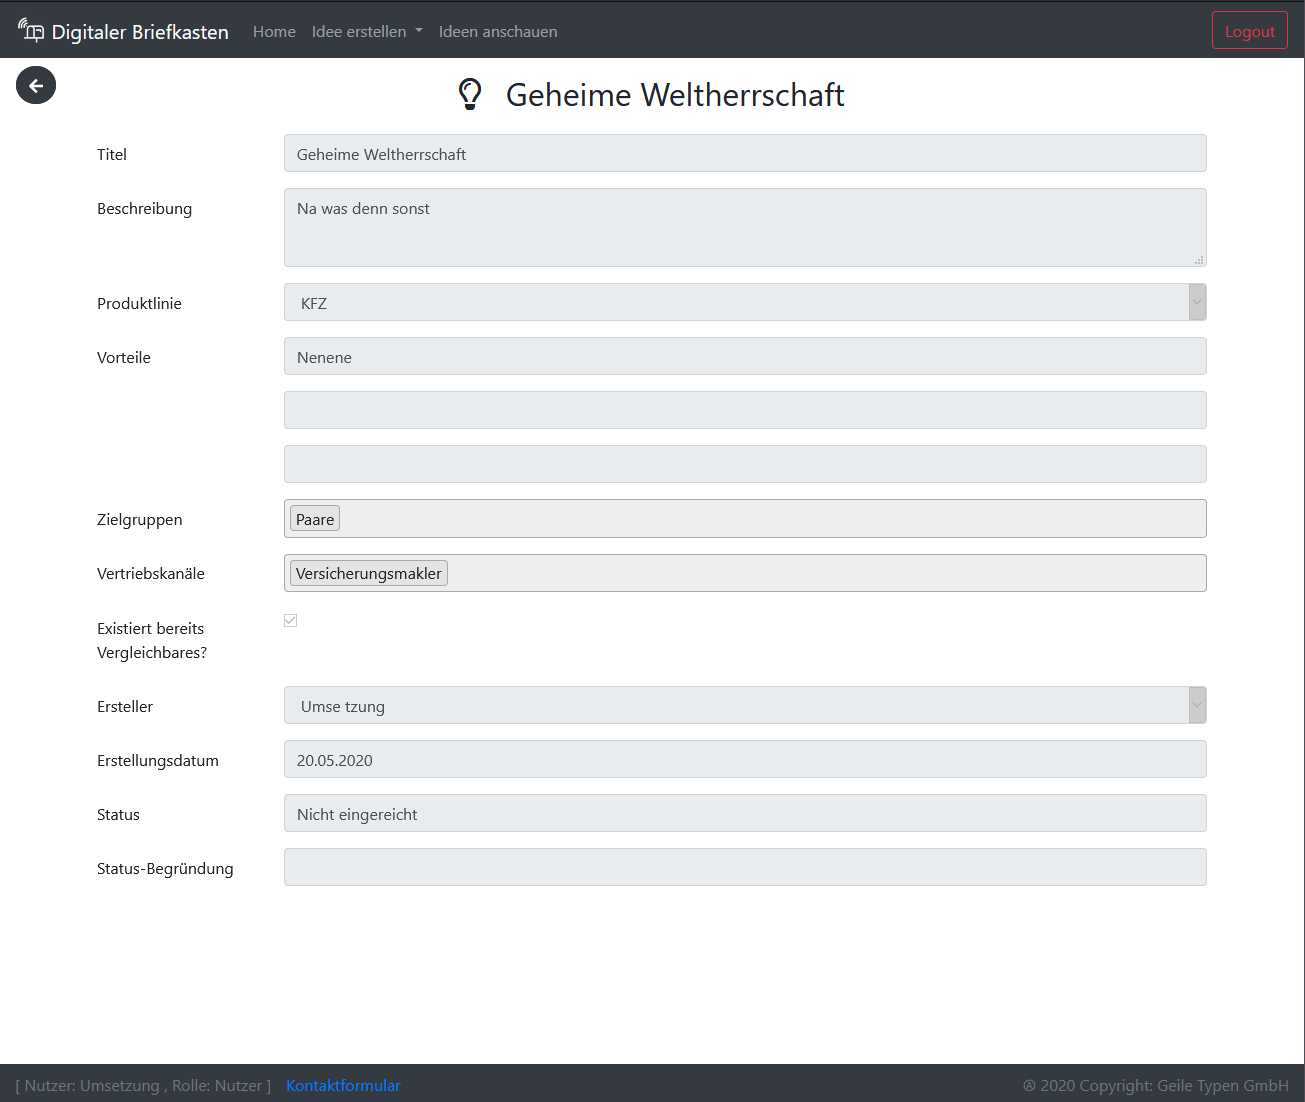
\includegraphics[width=1\textwidth]{img/idee-umsetzung.png}\\
        \source{Eigene Darstellung}
    \end{minipage}
\end{figure}

\begin{figure}[h]
    \centering
    \begin{minipage}[t]{1\textwidth}
        \caption{GUI-Umsetzung - Admin Ansicht }
        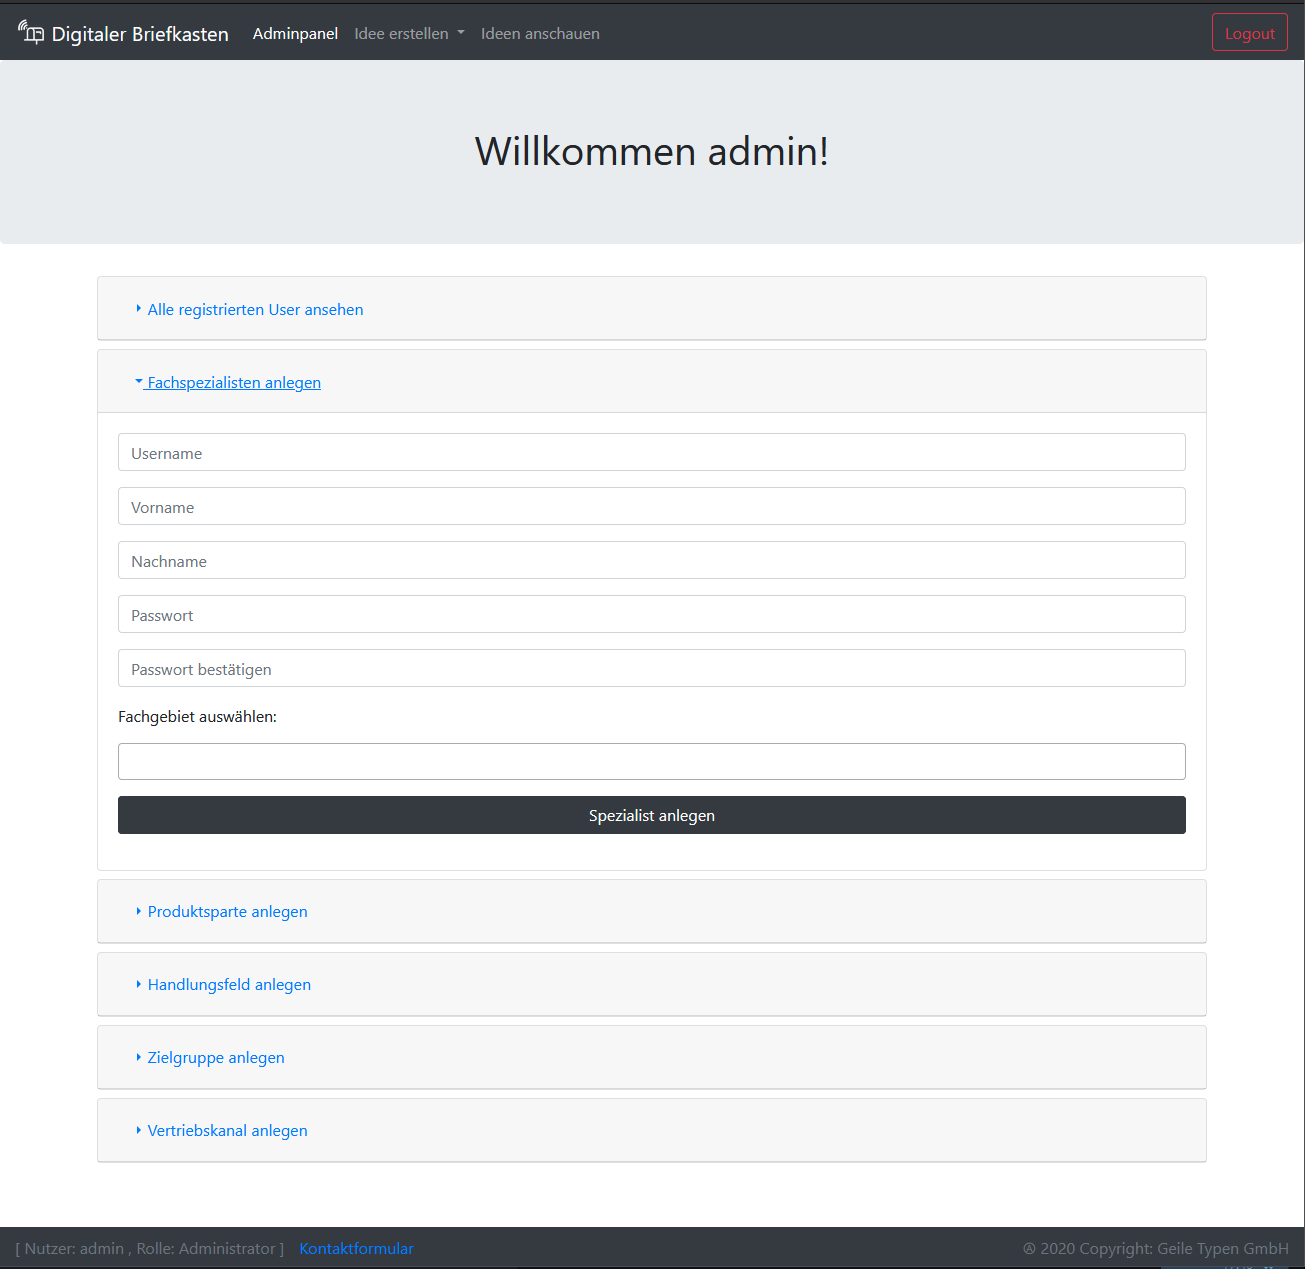
\includegraphics[width=1\textwidth]{img/admin-umsetzung.png}\\
        \source{Eigene Darstellung}
    \end{minipage}
\end{figure}

\begin{figure}[h]
    \centering
    \begin{minipage}[t]{1\textwidth}
        \caption{GUI-Umsetzung - Spezialist Ansicht }
        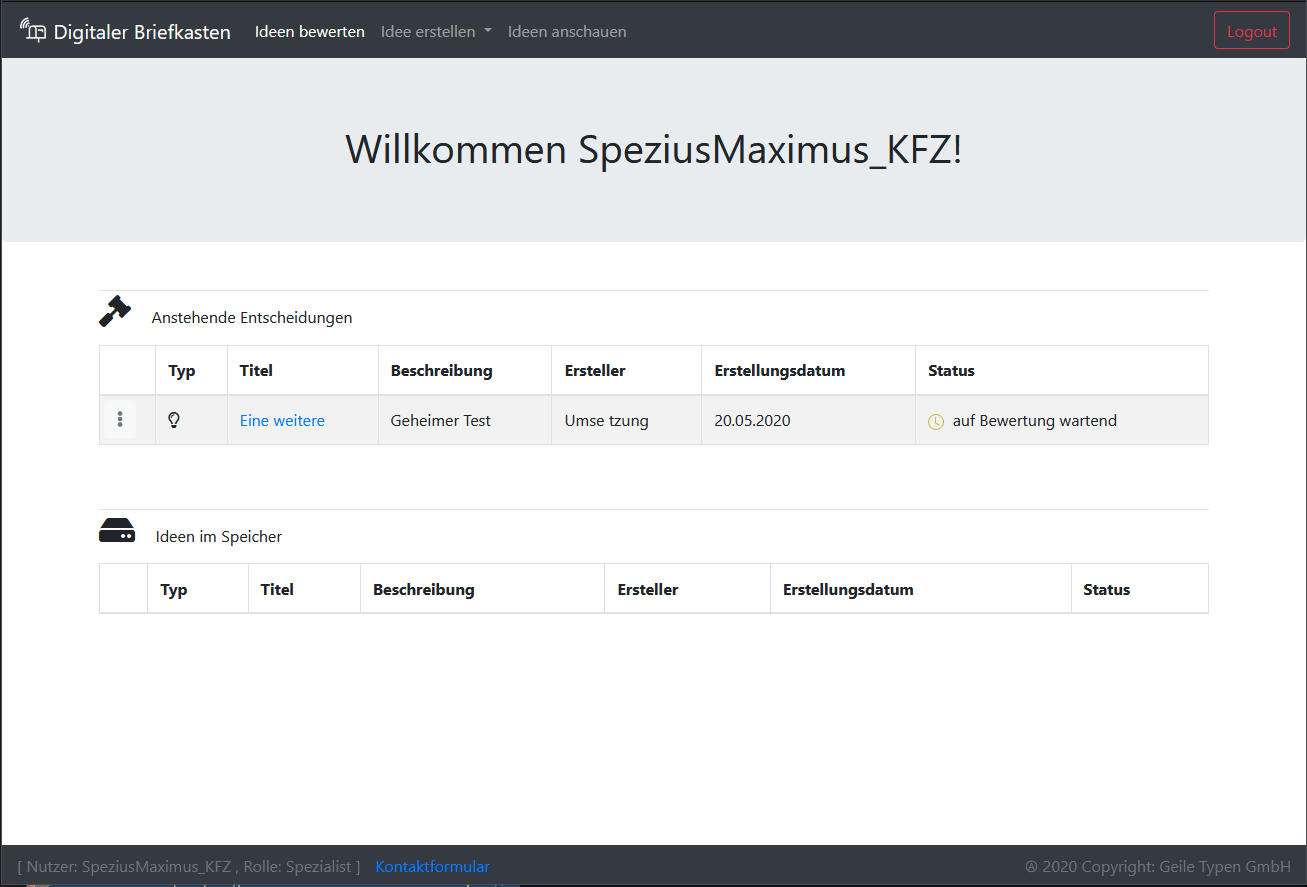
\includegraphics[width=1\textwidth]{img/spezialist-umsetzung.png}\\
        \source{Eigene Darstellung}
    \end{minipage}
\end{figure}

\pagebreak
\clearpage

\anhang{Projektplanung}
\subanhang{Projektstrukturplan}
\label{PSP}
\begin{figure}[h]
    \centering
    \begin{minipage}[t]{1\textwidth}
        \caption{Projektstrukturplan}
        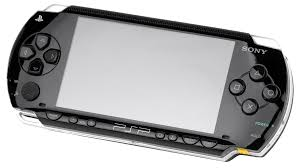
\includegraphics[width=1\textwidth]{img/psp.jpg}\\%TODO Jonathan fix me - Pictures need to be commited...
        \source{Eigene Darstellung}
    \end{minipage}
\end{figure}

\pagebreak
\clearpage
\begin{center}
    \begin{tabularx}{\linewidth}{
        |p{\dimexpr.09\linewidth-2\tabcolsep-1.3333\arrayrulewidth}% column 2
        |p{\dimexpr.61\linewidth-2\tabcolsep-1.3333\arrayrulewidth}% column 1
        |p{\dimexpr.3\linewidth-2\tabcolsep-1.3333\arrayrulewidth}|% column 3
    }
        \hline
        & Anforderung & Umsetzung \\ \hline
        Muss & Noch nicht registrierte Mitarbeiter können sich am System registrieren & Umgesetzt \\ \hline
        Muss & Registrierte Mitarbeiter können sich am System anmelden & Umgesetzt \\ \hline
        Muss & Registrierte Mitarbeiter können neue Ideen erfassen & Umgesetzt \\ \hline
        Muss & Registrierte Mitarbeiter können sich eine Liste ihrer eingereichten Ideen anzeigen lassen & Umgesetzt \\ \hline
        Muss & Registrierte Mitarbeiter können ihre Ideen solange bearbeiten oder auch löschen solange dieses noch nicht zur Bewertung an einen Fachspezialisten übergeben wurden. & Umgesetzt \\ \hline
        Muss & Nicht registrierte Mitarbeiter können vorhandene Ideen lesen, sich eine Übersicht der Ideen anzeigen lassen und die Übersicht filtern & Umgesetzt \\ \hline
        Muss & Diese Funktionen stehen auch registrierten Mitarbeitern zur Verfügung & Umgesetzt \\ \hline
        Muss & Neue Ideen werden Fachspezialisten zur Bewertung zugeordnet & Umgesetzt \\ \hline
        Muss & Die Zuordnung erfolgt automatisch sobald die Idee vom registrierten Mitarbeiter zur Bewertung eingereicht wurde & Umgesetzt \\ \hline
        Muss & Fachspezialisten können eine Idee entweder annehmen, ablehnen oder für einen späteren Zeitpunkt in einen sog. Ideenspeicher überführen / sie aus dem Ideenspeicher zurückholen & Umgesetzt \\ \hline
        Muss & Fachspezialisten begründen ihre Entscheidung transparent und für alle sichtbar in der Anwendung & Umgesetzt \\ \hline
        Muss & Fachspezialisten können ihnen zugewiesene Ideen in einer Liste sehen und diese Liste filtern & Umgesetzt \\ \hline
    \end{tabularx}

    \pagebreak

    \begin{tabularx}{\linewidth}{
        |p{\dimexpr.09\linewidth-2\tabcolsep-1.3333\arrayrulewidth}% column 2
        |p{\dimexpr.45\linewidth-2\tabcolsep-1.3333\arrayrulewidth}% column 1
        |p{\dimexpr.45\linewidth-2\tabcolsep-1.3333\arrayrulewidth}|% column 3
    }
        \hline
        & Anforderung & Umsetzung \\ \hline
        Kann & REST-API & Teilweise umgesetzt, lauffähig und erweiterbar \\ \hline
        Kann & Kontaktformular auch unregistriert & Umgesetzt, erweiterbar um E-Mail-Einbindung \\ \hline
        Kann & Administrator verwaltet Benutzer & Umgesetzt, erweiterbar \\ \hline
        Kann & Dokumentenupload zu einer Idee & Nicht umgesetzt, mit Erweiterung der Datenbank umsetzbar \\ \hline
        Kann & Profilfoto & Nicht umgesetzt, mit Erweiterung der Datenbank umsetzbar \\ \hline
        Kann & Fachspezialist: E-Mail Benachrichtigung bei neuer Idee & Nicht umgesetzt, erfordert E-Mail-Einbindung \\ \hline
        Kann & Benutzer: E-Mail Benachrichtigung bei Änderung einer Idee & Nicht umgesetzt, erfordert E-Mail-Einbindung \\ \hline
        Kann & PDF-Report über erstellte Ideen quartalsweise & Nicht umgesetzt \\ \hline
    \end{tabularx}
\end{center}

